\documentclass[a4paper]{report}

%====================== PACKAGES ======================

\usepackage[french]{babel}
\usepackage[utf8x]{inputenc}
%pour gérer les positionnement d'images
\usepackage{float}
\usepackage{amsmath}
\usepackage{graphicx}
\graphicspath{ {figures/} }
\usepackage[colorinlistoftodos]{todonotes}
\usepackage{url}
%pour les informations sur un document compilé en PDF et les liens externes / internes
\usepackage{hyperref}
%pour la mise en page des tableaux
\usepackage{array}
\usepackage{tabularx}
%pour utiliser \floatbarrier
%\usepackage{placeins}
%\usepackage{floatrow}
%espacement entre les lignes
\usepackage{setspace}
%modifier la mise en page de l'abstract
\usepackage{abstract}
%police et mise en page (marges) du document
\usepackage[T1]{fontenc}
\usepackage[top=1.8cm, bottom=2cm, left=2cm, right=2cm]{geometry}
%Pour les galerie d'images
\usepackage{subfig}

%====================== INFORMATION ET REGLES ======================

%rajouter les numérotation pour les \paragraphe et \subparagraphe
\setcounter{secnumdepth}{4}
\setcounter{tocdepth}{4}

\hypersetup{							% Information sur le document
pdfauthor = {Fligght},			% Auteurs
pdftitle = {Comparateur de vol},			% Titre du document
pdfsubject = {JEE},		% Sujet
pdfkeywords = {Tag1, Tag2, Tag3, ...},	% Mots-clefs
pdfstartview={FitH}}					% ajuste la page à la largueur de l'écran
%pdfcreator = {MikTeX},% Logiciel qui a crée le document
%pdfproducer = {}} % Société avec produit le logiciel

%======================== DEBUT DU DOCUMENT ========================

\begin{document}

%régler l'espacement entre les lignes
\newcommand{\HRule}{\rule{\linewidth}{0.5mm}}


%page de garde
\begin{titlepage}
\begin{center}

% Upper part of the page. The '~' is needed because only works if a paragraph has started.
%\includegraphics[width=0.35\textwidth]{./logo}~\\[1cm]
\begin{subfigure}{\textwidth}
  
\includegraphics[width=.15\linewidth]{./ensias.jpg}
\end{subfigure} \hfill
\begin{subfigure}{\textwidth}
  
\includegraphics[width=0.2\linewidth ]{./um5.png}
\end{subfigure}


    %
\includegraphics[width=0.16\textwidth]{logos/ensias.jpg}\par\vspace{1cm}
	 %\flushright
	%
\includegraphics[width=0.2\textwidth]{logos/um5.png}\par\vspace{1cm}
	%\flushleft
	\vspace{1cm}
	\centering %Centraliser le contenu	
	\newline
	\centering {\scshape\UE \\ Université Mohammed V \par}	
	\newline
	{\scshape\LARGE École Nationale Supérieure d'Informatique et d'Analyse des Systèmes \par} %Nom de l'université
	\vspace{3cm}

\textsc{\LARGE Rapport de Projet JAVA EE}\\[0.3cm]
\textsc{\large Génie Logiciel}\\[1.5cm]

\textsc{\Large }\\[0.5cm]

% Title
\HRule \\[0.4cm]

{\huge \bfseries Comparateur de Vol - Fligght\\[0.4cm] }

\HRule \\[1.5cm]
\vspace{3cm}
% Author and supervisor
\begin{minipage}{0.4\textwidth}
\begin{flushleft} \large
\emph{Elèves:}\\
\textsc{Bougtib Hafsa }\\
\textsc{Bouchrit Hamza }\\
\textsc{Chichi Amine }\\
\textsc{Abdeljalil Heggour}\\
\textsc{Fakhri Mouad}\\
\end{flushleft}
\end{minipage}
\begin{minipage}{0.4\textwidth}
\begin{flushright} \large
\emph{Encadrant:} \\
M. Mahmoud \textsc{EL HAMLAOUI}\\
\end{flushright}\\
\end{minipage}
\newline
\vspace{5cm}
% Bottom of the page
{\large Année Universitaire: 2020-2021}

\end{center}
\end{titlepage}
%page blanche
\newpage
~
%ne pas numéroter cette page
\thispagestyle{empty}


\Large
\renewcommand{\abstractname}{Remerciements}
\renewcommand{\abstractnamefont}{\normalfont\LARGE\bfseries}
%\renewcommand{\abstracttextfont}{\normalfont\Huge}

\begin{abstract}

\hskip7mm
\vspace{1cm}
\begin{spacing}{1}



~~~~Avant tout développement sur ce projet, nous souhaitons adresser mes remerciements les plus sincères aux personnes qui nous ont apporté leur aide et qui ont contribué à la réalisation de ce stage . Nous ne pourrions commencer ce rapport sans présenter nos remerciements les plus loyales à :\\



~~~~\textbf{Mr. Hamlaoui} , qui nous a encadré et accompagné tout au long de mon travail avec beaucoup de patience et de pédagogie, et qui n’a cessé de nous guider.\\




~~~~Nous n’oublions pas nos \textbf{membres de team} pour leur contribution, leur soutien et leur patience.\\

\end{spacing}
\end{abstract}

\renewcommand{\abstractname}{Résumé}
\renewcommand{\abstractnamefont}{\normalfont\LARGE\bfseries}
%\renewcommand{\abstracttextfont}{\normalfont\Huge}

\begin{abstract}
\hskip7mm
\vspace{1cm}
\begin{spacing}{1}

\Large {
Le présent document constitue le rapport de notre travail dans le cadre du \newline
Projet JEE, dont l’objectif est le développement d'un \textbf{"Comparateur de Vols"}.
\\ \par
Ce projet a comme objectif de permettre la comparaison des offres de vols des compagnies aériennes pour présenter aux utilisateurs les meilleures offres et possibilités de flight qu'ils cherchent selon leurs besoins et conditions horaires et financières .
\\ \par
Afin de le réaliser nous sommes passés par plusieurs phases : une première phase d’étude du contexte théorique et aspect technique du sujet, une deuxième phase d'analyse et de conception dans laquelle on a pu tester les différentes approches permettant de concevoir et résoudre le problème, puis une troisième phase de finalisation du projet et de présentation des résultats. Nous présenterons donc tout au long de ce rapport, les étapes que nous avons suivi ainsi que les outils que nous avons utilisé pour réaliser ce projet.


\vspace{10mm}
Mots Clés: \\
\newline
\indent \indent JEE - API - Tests - Comparaison

}
\end{spacing}
\end{abstract}

\renewcommand{\abstractname}{Abstract}
\renewcommand{\abstractnamefont}{\normalfont\LARGE\bfseries}
%\renewcommand{\abstracttextfont}{\normalfont\Huge}

\begin{abstract}
\hskip7mm
\vspace{1cm}
\begin{spacing}{1}

\Large {
This document is the report of our work on the JEE Project, whose objective is the development of a  \textbf{Flight Comparator}.
\\ \par
The main objectif of this project is to enable the comparison of airline flight offers, to present users with the best flight deals and opportunities they seek according to their needs and schedule and financial conditions.
\\ \par
In order to achieve this, we went through several phases : a first phase of study of the theoretical context and technical aspects of the subject, a second phase of design in which we were able to test the different approaches to solving the problem, then a third phase of project finalisation and presentation of results. We will therefore present throughout this report, the steps we followed as well as the tools we used to carry out this project.

\vspace{10mm}
Keywords: \\
\newline
\indent \indent JEE - API - Tests - Comparaison
}
\end{spacing}
\end{abstract}

\setcounter{page}{5}
%Liste des abréviations
%\addcontentsline{toc}{part}{Liste des abréviations}
\begin{center}
\vspace{7cm}    
\textbf{Liste des abréviations }
\vspace{2cm}
\setlength{\arrayrulewidth}{0.5mm}
\setlength{\tabcolsep}{18pt}
\renewcommand{\arraystretch}{2}

%{\rowcolors{3}{blue!50!white!30}{blue!50!white!20}
\begin{tabular}{ |p{7cm}|p{7cm}|p{7cm}|  }
%\hline
%\multicolumn{2}{|c|}{\textbf{Liste des abréviations }} \\
\hline
\textbf{Abréviation} & \textbf{Signification} \\
\hline
JEE & Java Entreprise Edition \\
HTML & Hypertext Markup Language \\
CSS & Cascading Style Sheet \\
JS & Javascript  \\
UML & Unified Modeling Language\\
\hline
\end{tabular}
%}



\end{center}

%\thispagestyle{empty}
\listoffigures
%\thispagestyle{empty}

\newpage
%\thispagestyle{empty}
\tableofcontents
%\thispagestyle{empty}
%ne pas numéroter le sommaire

\chapter*{Introduction Générale}
\addcontentsline{toc}{chapter}{Introduction Générale}


\\ L'idée du projet est basé sur une plateforme de comparaison des vols des compagnies aériennes . En effet , ceci va regrouper plusieurs compagnies aériennes pour permettre à l'utilisateur d'avoir la meilleure option pour son vol , dépendament des détails qu'il souhaite.
\\ \par
Ceci va être basé sur une comparaison des offres de ces compagnies aériennes , et lier par la suite ce client vers le site de cette dernière selon l'offre qu'il a choisi . \\

\\ \par
Notre document a pour objectif de présenter ce projet réalisé en équipe. Les phases de déroulement de ce projet sont structurées de la façon
suivante :
\\ \par
Le \textbf{premier chapitre} donne une partie présentation de "Fligght".

Le \textbf{deuxième chapitre} présente la partie Conception. 

Le \textbf{troisième chapitre} est consacré à la réalisation de l'application, ainsi qu'une description de la démarche suivie pour la conduite du projet.

\vspace{2cm}
Enfin, la conclusion générale présente une récapitulation des principaux résultats obtenus et
les perspectives du projet. 
\makeatletter
\renewcommand{\thesection}{\@arabic\c@section}
\makeatother

\newpage

%espacement entre les lignes d'un tableau
\renewcommand{\arraystretch}{1.5}

%====================== INCLUSION DES PARTIES ======================


~
\thispagestyle{empty}
%recommencer la numérotation des pages à "1"
%\setcounter{page}{0}
\newpage

\chapter{Présentation de la plateforme Fligght}

%Intro\footnotemark\\
\begin{spacing}{1.2}
%note en bas de page

\section{Introduction}

\par Ce chapitre introductif a pour objet de décrire la plateforme et son processus principal de comparaison.
%\begin{figure}[!h]
%\begin{center}
%remplacer "width" par "height" pour régler la hauteur
%\includegraphics[width=15cm]{presentation/schema}
%\end{center}
%légende de l'image
%\caption{Schéma descriptif}
%\end{figure}


\section{Présentation de "Fligght"}
La platforme est basée sur une api pour pouvoir accéder aux informations nécessaires sur les vols et les afficher au utilisateur.
Cette affichage est basé sur les filtres que ce dernier a choisi pour le vol désiré .
\\ \par
D'un point de vue utilisateur , ce dernier saisie en accédant à la plateforme toutes les informations qu'il souhaite a propos de son vol, pour que par la suite , toutes les vols qui sont convenables avec le résultat de recherche et comparaison s'affichent. 
\\ \par Ensuite , parmi ces résultats ce dernier présente le meilleur offre qui soit convenable avec ses critères , pour pouvoir lui lier à l'offre détaillée qui pourra par la suite la réserver sur le site officiel de la compagnie . Fligght inclue tous les vols que l'utilisateur cherchera , selon les possibilités horaires et budgétaires qu'il pourra chercher, tout dépendamment des offres annoncées par les compagnies responsables .

\end{spacing}
\newpage \par
\section{Conclusion}A propos du cycle de l'application , on peut dire que la tache déclenchante c'est celle de la saisie des informations du vol , puis recherche et comparaison , pour avoir les résultats qui lient l'utilisateur aux sites officiels des compagnies pour la réservation . Notre plateforme est censée en production inclure plus qu'une compagnie aérienne , mais pour ce projet on se limitera à une seule .

\chapter{Analyse et Conception}

\section{Introduction}
Le but de ce chapitre est de faire un cadrage technique et fonctionnel de notre projet. Nous allons présenter la démarche du de conception suivie, les besoins fonctionnels et non fonctionnels de notre projet, ainsi les diagrammes de cas d'utilisation réalisés.



\section{Besoin fonctionnels}
Il s’agit des fonctionnalités du système. Ce sont les besoins spécifiant un comportement d’entrée / sortie du système.

Afin d’obtenir une vue globale sur les exigences de l’application et ainsi réussir une bonne spécification des besoins, ces derniers doivent être modélisés. Nous avons donc eu recours aux concepts d’UML (Unified Modeling Language) pour représenter l'architecture et le fonctionnement de différentes fonctionnalités grâce à un ensemble de diagrammes très explicites.

\section{Besoin non fonctionnels}
Il s’agit des besoins qui caractérisent le système. Ce sont des besoins en matière de performance, de type de matériel ou le type de conception. Ces besoins peuvent concerner les contraintes d’implémentation. Ils agissent de façon indirecte sur le résultat et sur le rendement de l’application, ce qui fait qu’ils ne doivent pas être négligés, pour cela il faut répondre aux exigences suivantes :

\subsection{Fiabilité :}
La plateforme doit fonctionner de façon cohérente sans erreurs et doit être satisfaisante.
\subsection{Les erreurs :}
Les ambigüités doivent être signalées par des messages d’erreurs bien organisés pour bien guider l’utilisateur et le familiariser avec notre application.
\subsection{Ergonomie et bonne interface :}
L’application doit être adaptée à l’utilisateur dans toutes les résolution d’écran sans qu’il ne fournisse aucun effort (utilisation claire et facile) de point de vue navigation entre les différentes pages, couleurs et mises en textes utilisés.
\subsection{Sécurité :}
Notre solution doit respecter surtout la confidentialité des données personnelles des clients qui reste l’une des contraintes les plus importantes dans ces plateformes.
\subsection{Aptitude à la maintenance et la réalisation :}
Le système doit être conforme à une architecture standard et claire permettant sa maintenance et sa réutilisation.




\section{Diagramme de cas d'utilisation} \\
Les diagrammes de cas d'utilisation modélisent le comportement d'un système et permettent de capturer ses exigences. Ils décrivent aussi les fonctions générales et la portée d'un système.
\begin{figure}[!h]
\begin{center}
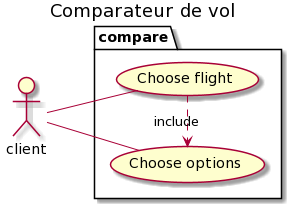
\includegraphics[height=8cm]{Pictures/Use case.png}
\end{center}
\caption{Diagramme de cas d'utilisation}
\end{figure}

\newpage
\section{Diagramme de classe}
Le diagramme de classes représente les classes intervenant dans le système. Le diagramme de classes est une représentation statique des éléments qui composent un système et de leurs relations

\begin{figure}[!h]
\begin{center}
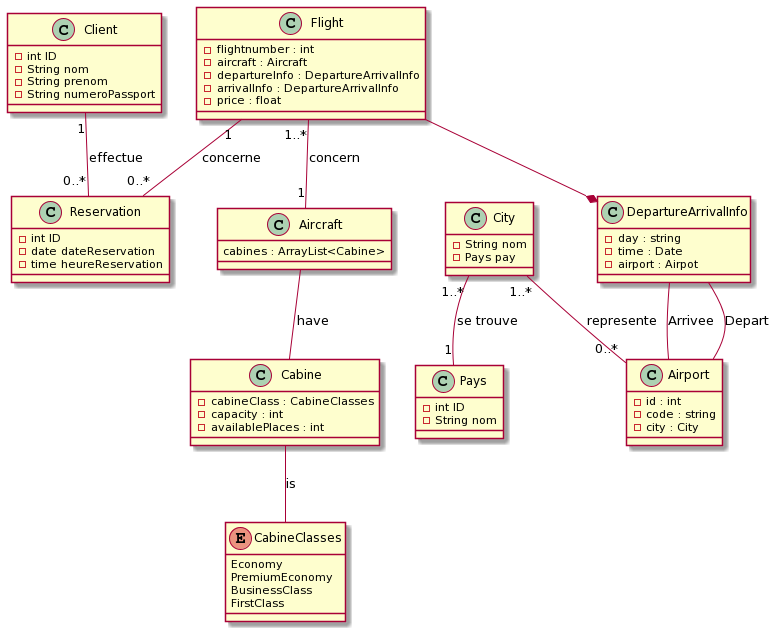
\includegraphics[height=8cm]{Pictures/Diag de classe.png}
\end{center}
\caption{Diagramme de classe}
\end{figure}
\section{Conclusion}

\\ L’analyse fonctionnelle est une démarche qui consiste à rechercher et à caractériser les fonctions offertes par un produit pour satisfaire les besoins de son utilisateur. Ce chapitre nous a permis de bien décrire le comportement de notre projet du point de vue de l’utilisateur en étudiant les besoins fonctionnels et non fonctionnels ainsi les diagrammes Classes et Cas d'utilisation.
 
\chapter{Réalisation}


\section{Introduction}
Cette partie constitue le dernier volet de ce rapport. Après avoir terminé la phase de l'analyse et la conception, nous présentons les outils et l’environnement logiciel de développement utilisés ainsi que les différents captures du projet.\\
\section{Outils et technologies}
\subsection{Langage de programmation}
Java Platform, Enterprise Edition ou Java EE, est une spécification pour la plate-forme Java d'Oracle, destinée aux applications d'entreprise.
La plate-forme étend Java Platform, Standard Edition (Java SE) en fournissant une API de mapping objet-relationnel, des architectures distribuées et multitiers, et des services web3. La plate-forme se fonde principalement sur des composants modulaires exécutés sur un serveur d'applications.\\
\begin{figure}[!h]
\begin{center}

\includegraphics[height=3cm]{Pictures/jee.png}
\end{center}
\caption{Logo Java EE}
\end{figure}

\\ \par 
GlassFish est un projet de serveur d'applications de plateforme open source Jakarta EE lancé par Sun Microsystems, alors sponsorisé par Oracle Corporation, et résidant désormais à la Fondation Eclipse et soutenu par Payara, Oracle et Red Hat. La version prise en charge sous Oracle s'appelait Oracle GlassFish Server
\\
\begin{figure}[!h]
\begin{center}

\includegraphics[height=4cm]{Pictures/glassfish.png}
\end{center}
\caption{Logo Glassfish}
\end{figure}

\\ \par 
HTML est un langage dit de « marquage », de « structuration » ou de « balisage » dont le rôle est de formaliser l’écriture d’un document avec des balises de formatage. Les balises permettent d’indiquer la façon dont doit être présenté le document et les liens qu’il établit avec d’autres documents.
\\
\begin{figure}[!h]
\begin{center}

\includegraphics[height=3cm]{Pictures/HTML.png}
\end{center}
\caption{Logo HTML}
\end{figure}

\\ \par 
Les feuilles de style en cascade, généralement appelées CSS de l'anglais Cascading Style Sheets, forment un langage informatique qui décrit la présentation des documents HTML et XML. Les standards définissant CSS sont publiés par le World Wide Web Consortium (W3C). Introduit au milieu des années 1990, CSS devient couramment utilisé dans la conception de sites web et bien pris en charge par les navigateurs web dans les années.
\\
\begin{figure}[!h]
\begin{center}

\includegraphics[height=3cm]{Pictures/css.png}
\end{center}
\caption{Logo CSS}
\end{figure}

\\ \par 
JavaScript est un langage de programmation qui permet d’implémenter des mécanismes complexes sur une page web. À chaque fois qu’une page web fait plus que simplement afficher du contenu statique — afficher du contenu mis à jour à des temps déterminés, des cartes interactives, des animations 2D/3D, des menus vidéo défilants, etc... — JavaScript a de bonnes chances d’être impliqué. C’est la troisième couche des technologies standards du web, les deux premières (HTML et CSS).
\\
\begin{figure}[!h]
\begin{center}

\includegraphics[height=3cm]{Pictures/js.png}
\end{center}
\caption{Logo JavaScript}
\end{figure}


%\cite{cite2} 
%---------------Environnement de développement------------------
\subsection{Environnement de développement}
Docker est un ensemble de produits de plate-forme en tant que service (PaaS) qui utilisent la virtualisation au niveau du système d'exploitation pour fournir des logiciels dans des packages appelés conteneurs. Les conteneurs sont isolés les uns des autres et regroupent leurs propres logiciels, bibliothèques et fichiers de configuration; ils peuvent communiquer entre eux via des canaux bien définis. Étant donné que tous les conteneurs partagent les services d'un seul noyau de système d'exploitation, ils utilisent moins de ressources que les machines virtuelles.
\\
\begin{figure}[!h]
\begin{center}

\includegraphics[height=3.5cm]{Pictures/docker.png}
\end{center}
\caption{Logo Docker}
\end{figure}
\newline
\\ \par 
Maven est un puissant outil de gestion de projet basé sur POM (Project Object Model). Il est utilisé pour la construction de projets, les dépendances et la documentation. Cela simplifie le processus de construction comme ANT. Mais c'est trop avancé que ANT.\newline
En bref, nous pouvons dire que maven est un outil qui peut être utilisé pour créer et gérer n'importe quel projet basé sur Java. maven facilite le travail quotidien des développeurs Java et aide généralement à la compréhension de tout projet basé sur Java.
\\
\begin{figure}[!h]
\begin{center}

\includegraphics[height=2.5cm]{Pictures/maven.png}
\end{center}
\caption{Logo Maven}
\end{figure}

\subsection{Gestion de version et de collaboration}
Git est un logiciel de gestion de versions décentralisé. C'est un logiciel libre créé par Linus Torvald, auteur du noyau Linux, et distribué selon les termes de la licence publique générale GNU version 2. En 2016, il s'agit du logiciel de gestion de versions le plus populaire qui est utilisé par plus de douze millions de personnes.
\\
\begin{figure}[!h]
\begin{center}

\includegraphics[height=3cm]{figures/git.png}
\end{center}
\caption{Git}
\end{figure}



%---------------Communication------------------
\subsection{Outils de Communication}
Google Meet est un service de video conférence developpé par Google. Il est utilisé au sein de l'entreprise Daba'Go pour effectué des réunions avec des partenaires aussi bien une réunion pour tous les collaborateurs, elle est toujours programmée chaque vendredi après-midi pour se rencontrer tous et discuter les avancements dans chaque équipe.
\\
\begin{figure}[!h]
\begin{center}

\includegraphics[height=1cm]{figures/google_meet_logo.png}
\end{center}
\caption{Google Meet}
\end{figure}

\newpage
\section{Intérfaces}


\begin{figure}[htb!]
  \centering

\includegraphics[height=0.43\paperwidth,width=0.8\paperwidth]{Pictures/Home.png}
\caption{Page Home}
\end{figure}
\FloatBarrier

\begin{figure}[htb!]
  \centering
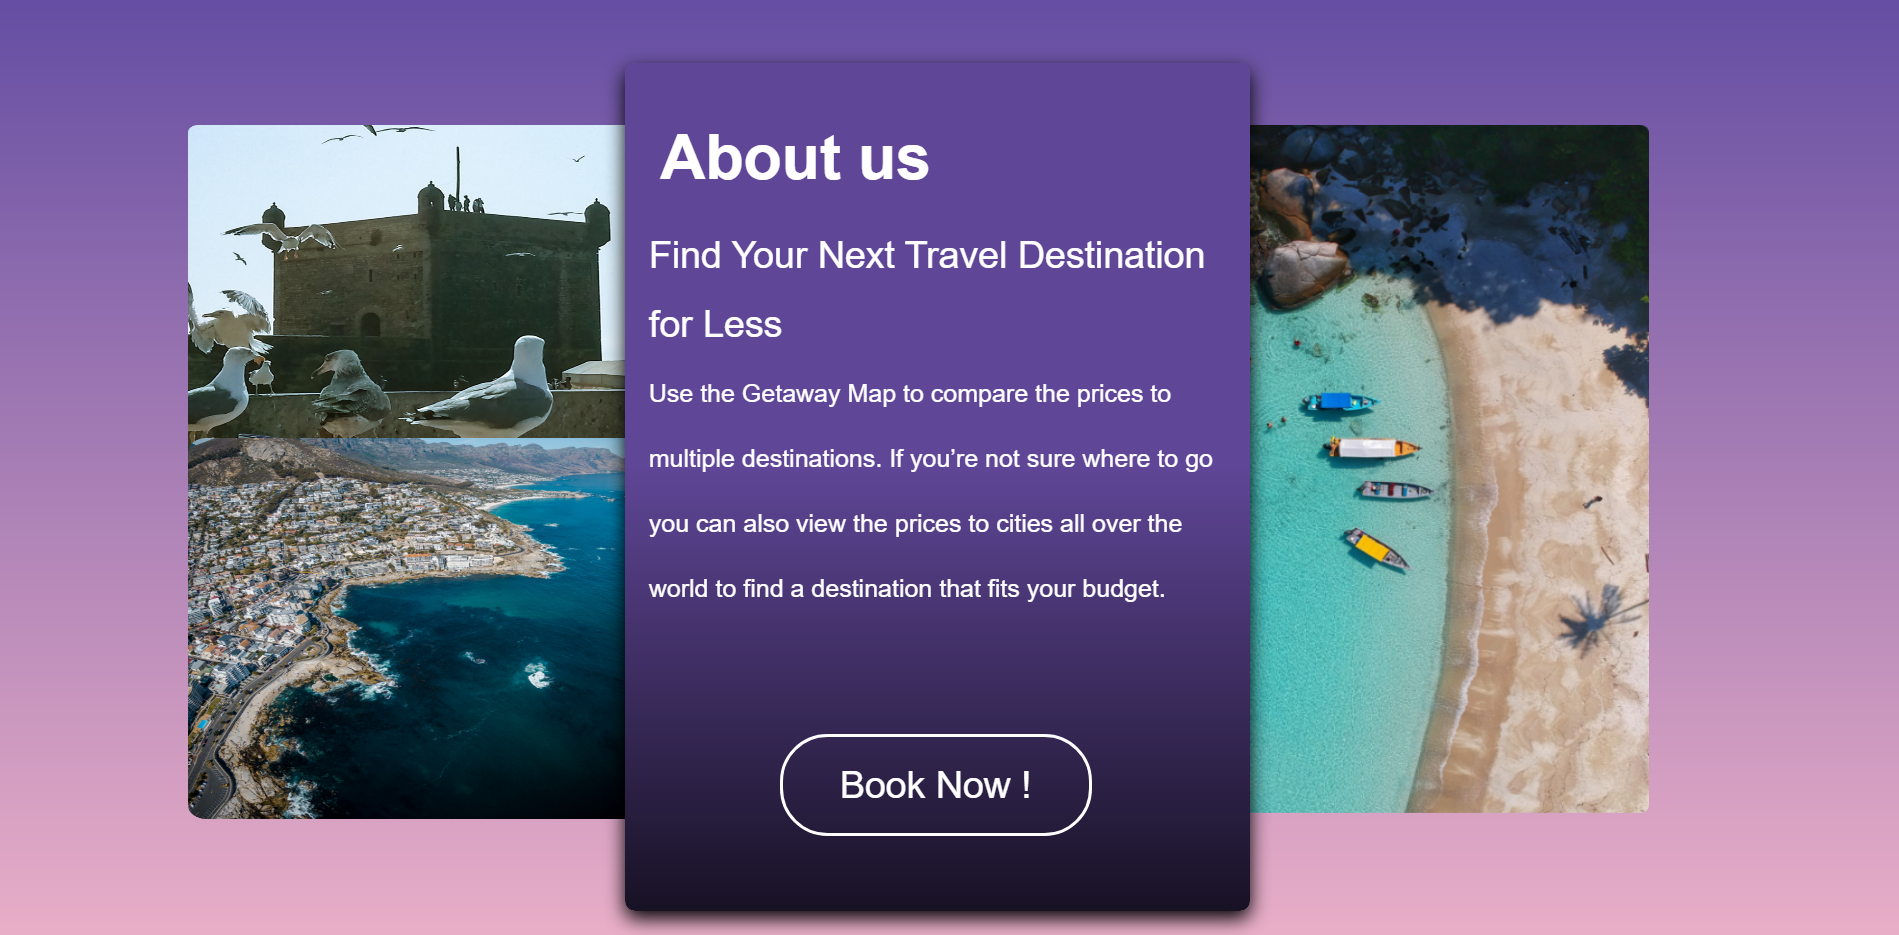
\includegraphics[height=0.43\paperwidth,width=0.8\paperwidth]{Pictures/About us.png}
\caption{About us}
\end{figure}
\FloatBarrier



\begin{figure}[htb!]
  \centering
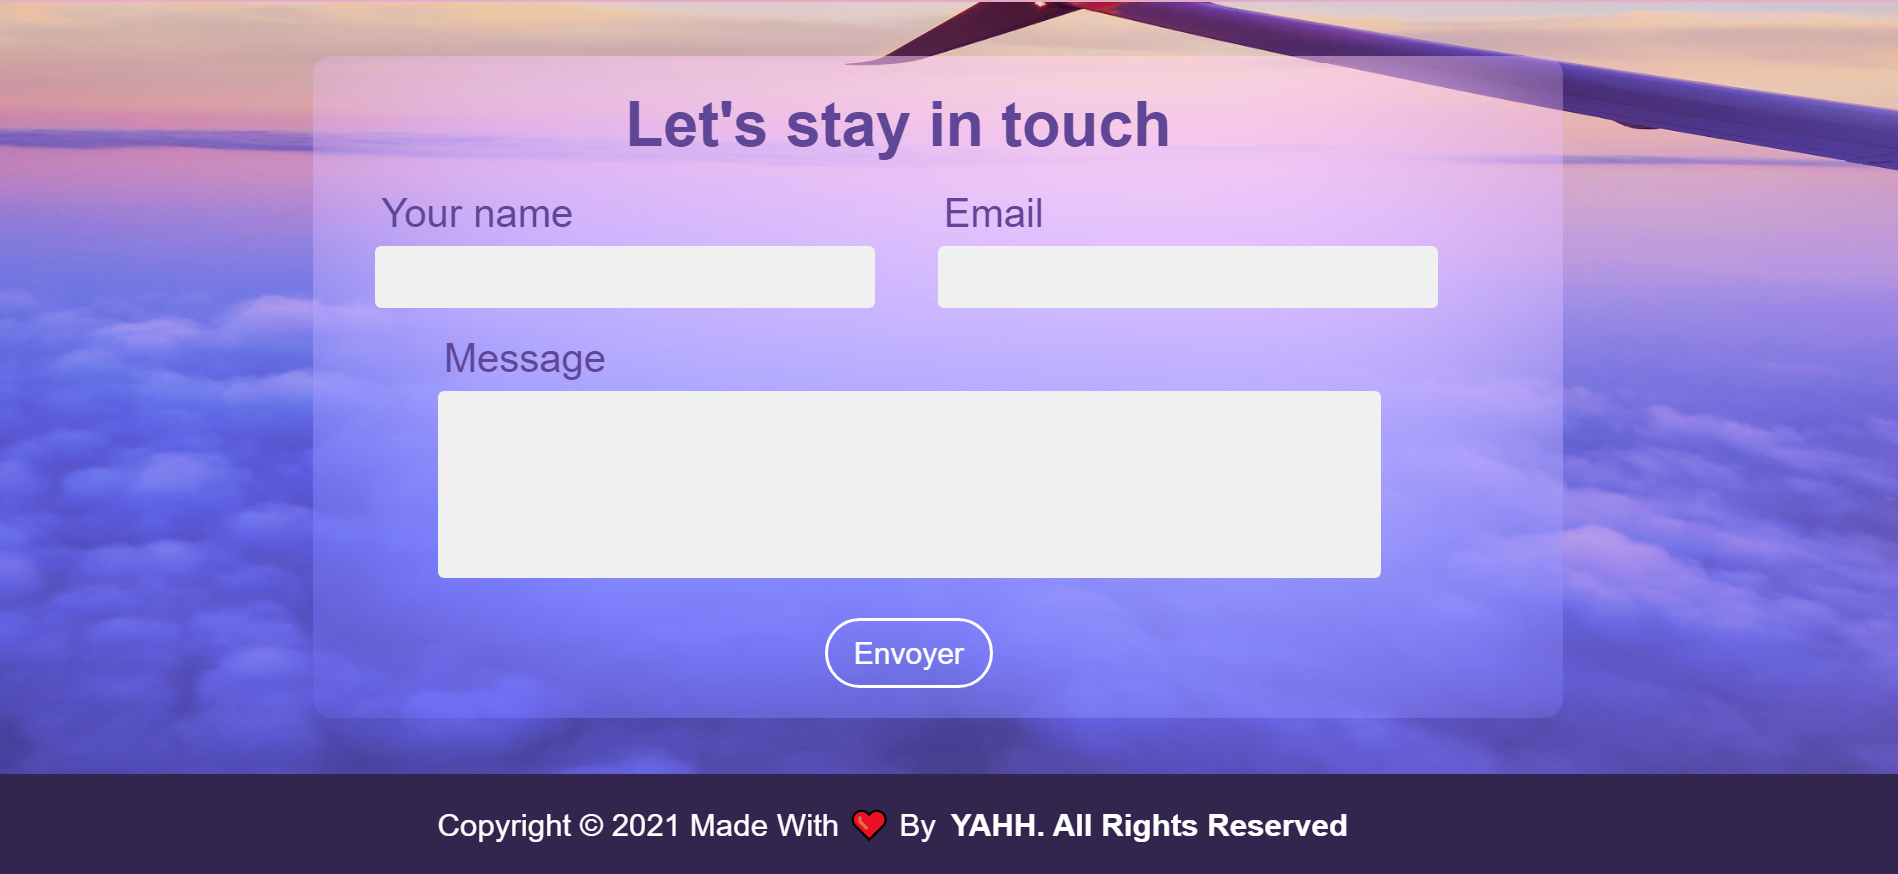
\includegraphics[height=0.43\paperwidth,width=0.8\paperwidth]{Pictures/Contact us.png}
\caption{Contact Us}
\end{figure}
\FloatBarrier


\begin{figure}[htb!]
  \centering

\includegraphics[height=0.43\paperwidth,width=0.8\paperwidth]{Pictures/Search.png}
\caption{Search for flights}
\end{figure}
\FloatBarrier

\begin{figure}[htb!]
  \centering
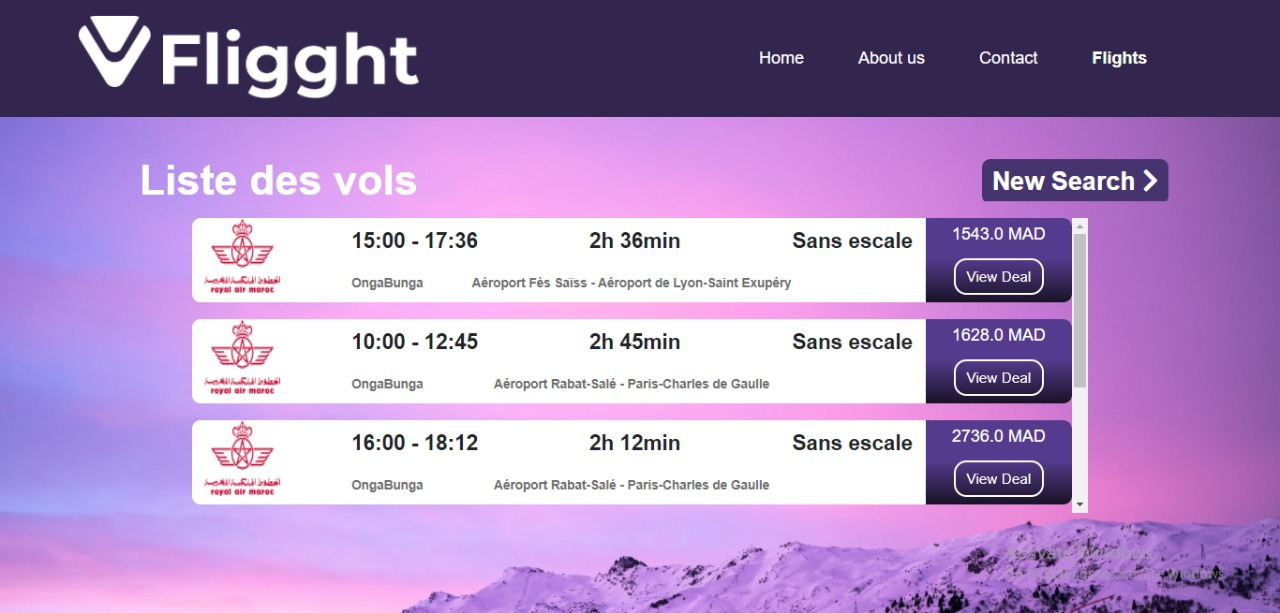
\includegraphics[height=0.43\paperwidth,width=0.8\paperwidth]{Pictures/Result.jpeg}
\caption{Search result}
\end{figure}
\FloatBarrier


%Ne pas numéroter cette partie
%\part*{Annexes}
%Rajouter la ligne "Annexes" dans le sommaire
\addcontentsline{toc}{part}{Conclusion}
\chapter*{Conclusion}
% \newpage
\vspace{2cm}
\par Tout au long de ce rapport, nous avons présenté la démarche que nous avons suivie pour mettre au point ce projet. Ainsi, l'analyse et la conception en étudiant les besoins et les scénarios de notre projet. Puis, la phase de développement qui nous a donné l’occasion de faire le lien entre les connaissances académiques, notamment la programmation Jee et découvrir de nouveaux outils tels que Docker, Junit .. etc\\

\par Ce projet nous a permis d’approfondir nos connaissances théoriques et pratiques notamment dans le domaine de développement des applications web. Ainsi, il a été aussi une belle occasion pour assurer un travail de groupe , même avec ces conditions non favorables.
\\ \par
Malgré les problèmes rencontrés durant la réalisation du stage notons le travail à distance comme étant l'obstacle majeur de notre projet puisque la mission était 100\% en ligne et on n'a pas eu la possibilité de se rencontrer, nous avons pu gérer la situation et trouver des solutions citant par exemple les réunions de mise en point plusieurs fois par semaine ainsi pour se rencontrer tous et discuter les avancements dans chaque membre.\\
\newpage
%\addcontentsline{toc}{part}{Bibliographie}
%\chapter*{Webographie}

\vspace{2cm}

\begin{itemize}
\\\item \textbf{\Large{Cours et documentations : }}\\
  [\url{https://openclassrooms.com/fr/courses/626954-creez-votre-application-web-avec-java-ee/}] \vspace{0.3cm}

\\{[2]} HeadFirst JAVA, auteurs : Bert Bates et Kathy Sierra 
\vspace{0.3cm}
\\{[3]} Documentation Android Studio :[ \url{https://developer.android.com/guide/}]
\vspace{0.3cm}
\\{[4]} Documentation Firebase :[ \url{https://firebase.google.com/docs/android/setup}]
\vspace{0.3cm}
\\{[5]} Documentation GoogleMaps : [ \url{https://developers.google.com/maps/documentation/android-sdk/map}]
\vspace{1cm}

\\ \item \textbf{\Large{Forums et Siteweb:}}\\
\\{[6]} Stackoverflow [\url{http://www.stackoverflow.com}]
\vspace{0.3cm}
\\{[7]} Medium [\url{https://medium.com}]

\vspace{1cm}
\\ \item \textbf{\Large{Chaînes Youtube :}}\\
\\{[8]} Firebase 
[\url{https://www.youtube.com/channel/UCP4bf6IHJJQehibu6ai__cg}]
\vspace{0.3cm}
\\{[9]} CodingWithMitch [\url{https://www.youtube.com/channel/UCoNZZLhPuuRteu02rh7bzsw}]\\
\\{[10]} Coding in Flow [\url{https://www.youtube.com/channel/UC_Fh8kvtkVPkeihBs42jGcA}]

\end{itemize}



%récupérer les citation avec "/footnotemark"
\newpage
\nocite{*}
\bibliographystyle{unsrt}
%inclusion de la biblio
\bibliography{biblio.bib}
\addcontentsline{toc}{chapter}{Bibliography}

\end{document}